%\{ {\it  sp1d\_ch3\_2.tex} \}

\begin{figure}[h]
    \begin{center}
    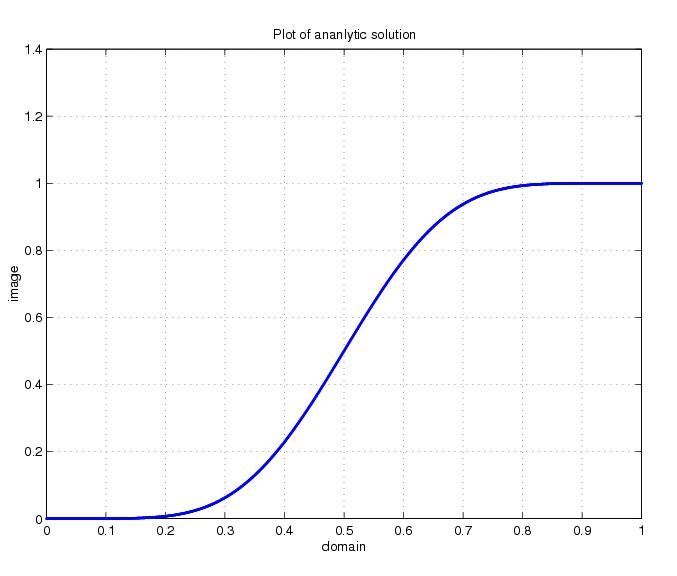
\epsfig{file = Doc-Report_Fwd1D/figs_dn/ScrvO_13.eps, width = 5cm}
    \caption{\label{scrvsol1}Example of a curve satisfing conditions (\ref{pois_scrv1}), with polynomial order $n=9$}.
    \end{center}
\end{figure}

\subsubsection {High order Polynomial Solution and Its Convergence}

In this section we construct a polynomial $P_n$ of order $n$ defined on $[0,1]$, which satisfies the following.
\begin{eqnarray}
\label{pois_scrv1}
    P_n(0) = 0, &P_n(1) = 1 \\
    \frac{d^k}{dx^k}P_n(0) = 0, &\frac{d^k}{dx^k}P_n(1) = 0
\end{eqnarray}
for all $k = 1, \cdots, n-2$. \\
For each $n$, we obtain a polynomial $P_n$ by solving a system of
linear equations that determines the coefficients of $P_n$. We
apply the spectral polynomial solver to approximate the second
derivative $Q_{n-2}$ of $P_n$. The numerical and exact solutions
by the solver we developed is shown in figure (\ref{scrvsol1}).



\begin{problem}
Consider the following differential equation for $u(x)$ such that
\begin{equation}
\label{poi_poly1}
    \frac{d^2}{dx^2} u(x) = Q_{n-2},
\end{equation}
for all $x$ in $[0, 1]$ with the boundary condition defined in
equation (\ref{pois_scrv1}). Approximate $u(x)$ using spectral
polynomial method.
\end{problem}

Note that the accuracy of the interpolation satisfying equations
(\ref{pois_scrv1}) is dependent on the stability of the matrix
defining the coefficients of interpolants. We used the Legendre
basis functions because they are known to be more stable than
monomials. Despite this choise, interpolation error is nearly
$e^{-13}$. This results in the same amount of convergence error in
p-type extension mode shown in right of Figure (\ref{ScrvconvDN1})
and Table (\ref{hconv2t1}).

\begin{enumerate}

\item {Convergence h-type extension for equation (\ref{poi_poly1})}
Examining the equation (\ref{pois_sin1}), in Figure
(\ref{ScrvconvDN1}), we observe that the error with respect to
$L^{\infty}$ of the discrete solution to the equation is
exponentially convergent with respect to the size of element. This
verifies the Log-Log scale of relation of theory
(\ref{hrelation}).
\item {Convergence p-type extension for equation (\ref{poi_poly1})}
This semi-Log scale plot also shows the exponential convergence of
p-type extension of trial functions. Note that we approximate the
finite order of the polynomials. So there exists the lowest order
$P_l$ that approximates with trial functions of order $P$ which $P
> P_l$ should shows the same convergence as the case using trial
functions of order $P_l$. In right of Figure (\ref{ScrvconvDN1}),
we observe that the convergence is staying on approximation error
which theoretically should be machine precision.
\end{enumerate}

\begin{figure}[h]
\begin{center}
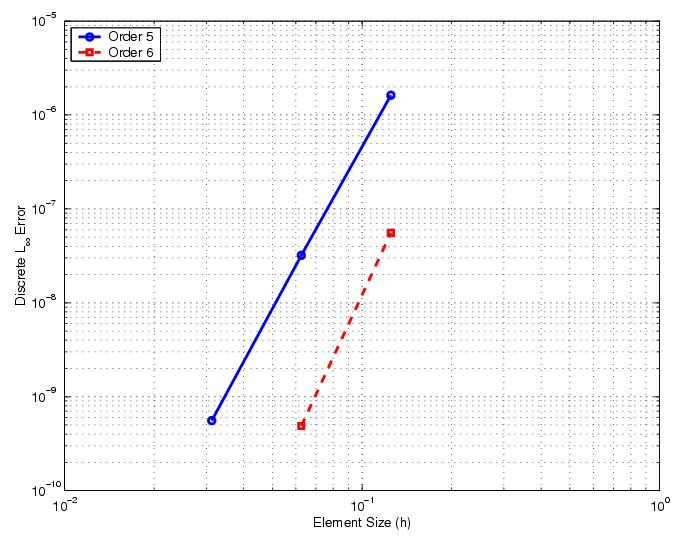
\epsfig{file = Doc-Report_Fwd1D/figs_dn/ScrvHconv.eps, width = 8.3cm}
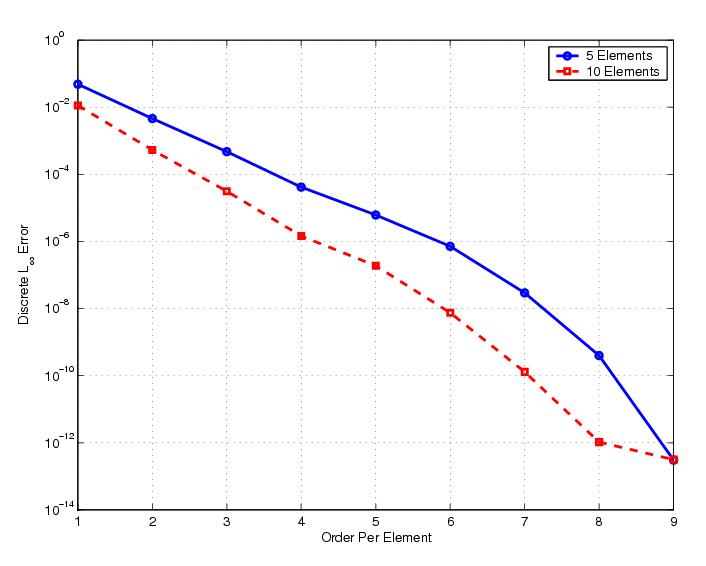
\epsfig{file = Doc-Report_Fwd1D/figs_dn/ScrvPconv.eps, width = 8.3cm}
\caption{\label{ScrvconvDN1}
(Left) Convergence with respect to discrete $L^{\infty}$ norm as a function of  element
size. This test is performed using the h-type extension with fixed
polynomial order 3, 4, and 5 respectively. Error on the Log-Log
axis demonstrates the algebraic convergence of the h-type
extension.
(Right) Convergence w.r.t. $L^{\infty}$ norm as a function of size
of polynomial order in semi-Log plot. It shows the exponential
convergence of p-type extension for smooth solution. The two tests
are performed for p-type extension with element lengths of $0.2$
and $0.1$. }
\end{center}
\end{figure}

\begin{table}[h]
\centering \caption{\label{hconv2t1} This table shows the
convergence of h-type resolution control done above Figure
(\ref{ScrvconvDN1}). Note that the slopes of each order $P$ is
$P+1$ }
\begin{tabular}{|c|c|c|} \hline
    Polynomial order&Error($L^{\infty}$)&Slope   \\ \hline \hline
    3&$7.5530e-011$ &$3.9908$ \\ \hline
    4&$4.5619e-013$ &$4.6486$ \\ \hline
    5&$4.1855e-013$ &$5.7218$ \\ \hline
\end{tabular}
\hspace{.5in}
\begin{tabular}{|c|c|} \hline
    &\multicolumn{1}{|c|}{Error}\\
    \raisebox{0.5\baselineskip}%
    {Element Size}&($L^{\infty}$) \\ \hline \hline
    0.2&$3.0431e-013$  \\ \hline
    0.1&$3.1186e-013$ \\ \hline
\end{tabular}
\end{table}
